\section{Messwerte und Auswertung} % (fold)
\label{sec:messwerte_und_auswertung}

	\subsection{Michelson-Interferometrie} % (fold)
	\label{sub:michelson_interferometrie}
	
		\subsubsection{Fizeau-Streifen und Haidinger Ringe} % (fold)
		\label{ssub:fizeau_streifen}

			Die Interferenzen gleicher Dicke wurden durch Verkippen von Spiegel 2 erzeugt.
			Dabei entstanden die horizontalen Streifen aus Abbildung \ref{fig:fizeau-h-1} durch Drehung um die horizontale (y-) Achse senkrecht zur Verschiebungsrichtung x.
			Analog ließen sich die vertikalen Interferenzmuster durch Drehung um die Vertikale, also die z-Achse bilden.
			Während man bei den senkrechten Interferenzmuster von Abbildung \ref{fig:fizeau-v} gerade Steifen erkennt, die zur Seite jedoch einen größeren Abstand aufweisen, sieht man die Streifen von Abbildung \ref{fig:fizeau-h-1} in annäherend gleichen Abstand, jedoch verzerrt.
			Beides spricht in diesem Fall für eine Spiegelkrümmung einer der beiden Spiegel in z-Achsen-Richtung.
		
			\begin{figure}[htb]
				\centering
				\includegraphics[scale=0.1]{messwerte/fizeau-streifen-h-1.png}
				\caption{Horizontale Fizeau-Streifen durch Interferenz der grünen Hg-Dampflinie bei $\lambda = 546 \unit{nm}$}
				\label{fig:fizeau-h-1}
			\end{figure}

			\begin{figure}[htb]
				\centering
				\includegraphics[scale=0.1]{messwerte/fizeau-streifen-v-1.png}
				\caption{Vertikale Fizeau-Streifen durch Interferenz der grünen Hg-Dampflinie bei $\lambda = 546 \unit{nm}$}
				\label{fig:fizeau-v}
			\end{figure}

			Mit Hilfe des Maxima-Abstandes und der unter \ref{sub:interferenzen_gleicher_dicke_fizeau_streifen} angegebenen Formel, kann man in etwa den Winkel der Verkippung aurechnen.
			Um die Abstände zu normieren wird angenommen, dass das Bild nur durch die letzte Linse vergrößert wird und somit der ursprüngliche Durchmesser des Bildes gleich dem Linsendruchmesser ist, welcher im Versuch zu $D = 3 \unit{cm} $ bestimmt wurde.
			Im Durchschnitt beträgt der Streifenabstand $a$ der senkrechten Streifen dann in etwa $a = 0.75 \unit{cm}$.
			\[ \implies \sin(\alpha /2) = \frac{\lambda}{2 a} = \frac{546 \unit{nm}}{2 \cdot 0.75 \unit{cm}} 
			\approx 3.64 \cdot 10^{-5} \]
			\[ \implies \alpha \approx 7.3 \cdot 10^{-5} = 15 "\]
			Betrachtet man den zweit untersten horizontalen Streifen in Abbildung \ref{fig:fizeau-h-1} dann beträgt die Höhendifferenz zwischen Mitte und Rand in etwa die gesamte Breite des Maximums.
			Folglich wird die Abweichung von der planen Fläche eines der beiden Spiegel auch in dem Bereich von $\lambda$ also etwa $0.5 \unit{$\mu$m}$ liegen.

			Die Haidinger-Ringe konnten mit etwas Feingefühl zwar eingestellt werden und zeigten auch das unter \ref{sub:interferenzen_gleicher_neigung_haidinger_ringe} gezeigte Verhalten, allerdings ließ sich aufgrund des schwachen Kontrastes und er geringen Leuchtstärke im Vergleich zu anderen Reflexen keine verwertbare Aufnahme anfertigen.


		% subsubsection fizeau_streifen (end)

		\subsubsection{Einlfuss der Glasplatte} % (fold)
		\label{ssub:einlfuss_der_glasplatte}

			Das MIF findet auch Anwedung bei der Bewertung der Güte optischer Bauteile.
			Als Beispiel wurde hier der Einfluss einer scheinbar planparallelen Glasplatte auf die Interferenzmuster untersucht.
			Dazu stellten wir zunächst eine möglichst geringe Spiegelverschiebung ein, also den Bereich der Haidinger-Ringe, zu erahnen in Abbildung \ref{fig:ohne_platte}.
			Als nächstes wurde die Platte in Strahlengang 2 gestellt.
			Wie man in Bild \ref{ sehen kann tauchen nun Fizeau-Streifen auf, was bedeutet, dass die Platte einen ähnlichen Einfluss wie die Spiegelverkippung hat.
			Daraus folgt, dass sie an einer Seite dicker sein muss als an der anderen und somit der optische Weg hier verlängert wird.
			Wie man in Aufnahme 56789 erkennt muss dies auf der asdfghjhgfd Seite der Fall sein.
			Das Erscheinen von 999 Streifen bedeutet eine maximale Wegdifferenz von $999 \lambda$.
			Für die Glasplatte bedeutet das eine Stärkendifferenz von:
			\[ \Delta d = \frac{999 \lambda}{2 (n_\m{Glas} - n_\m{Luft}) } == 895678 \]

			\begin{figure}[htb]
				\centering
				\includegraphics[scale=0.1]{messwerte/harded-fucked-in-budapest-1.png}
				\caption{}
				\label{fig:ohne_platte}
			\end{figure}

			\begin{figure}[htb]
				\centering
				\includegraphics[scale=0.1]{messwerte/harded-fucked-in-budapest-2-extended-unedited-directors-cut.png}
				\caption{}
				\label{fig:mit_platte}
			\end{figure}

		% subsubsection einlfuss_der_glasplatte (end)

		\subsubsection{Weißlichtinterferenz} % (fold)
		\label{ssub:wei_lichtinterferenz}

			Auch das Licht eines thermischen Strahlers kann am MIF zur Interferenz gebracht werden.
			In Abbildung 56789 ist dies zu sehen.
			Die Anforderung hierbei ist den sehr kleinen Bereich der Kohärenzlänge $l_\m{koh}$ genau einzustellen.
			Durch Verkippen von Spiegel 2 konnten wir nun wie im Bild zu erkennen maximal 999 Fizeau-Streifen erzeugen, bis die Wegdifferenz $2 \Delta x > l_\m{koh}$ war.
			Wenn wir für weißes Licht eine mittlere Wellenlänge von etwa $\overline{\lambda} = 550 \unit{nm} $ einsetzen erhalten wir als Abschätzung für die Kohärenzlänge:
			\[ l_\m{koh} = 999 * \overline{\lambda} == 897 \]

		% subsubsection wei_lichtinterferenz (end)


		\subsubsection{Inhomogener Brechungsindex durch Wärme} % (fold)
		\label{ssub:inhomogener_brechungsindex_durch_w_rme}
			
			Die Empfindlichkeit des MIF konnte im Versuch mit einem heißen Widerstand demonstriert werden.
			Der Widerstand wurde im Strahlgang vor Spiegel 2 positioniert und die Luft über ihm erwärmt.
			Daraus resultierte eine Verminderung des Brechungsindex, was zu einer Verkürzung der optischen Weglänge führt.
			In Abbildung \ref{fig:hot ohm} ist das Interferenzmuster mit eingebrachten Widerstand zu sehen.

			\begin{figure}[htb]
				\centering
				\includegraphics[scale=0.1]{messwerte/hot-ohm-a.png}
				\caption{Interferenzstreifen der grünen Hg-Dampflinie bei $\lambda = 546 \unit{nm}$ mit Wärmequelle im Strahlgang}
				\label{fig:hot ohm}
			\end{figure}

			Man sieht, dass die regelmäßigen Fizeau-Streifen im linken Bereich verzerrt sind.
			Hier ist der Strahl durch heißere Luft propagiert.
			Die maximale Verschiebung kann anhand der Abbildung auf etwa 999 geschätzte werden.
			Damit ergibt sich über den insgesamt etwa $2 \unit{cm} $ langen Widerstand eine Weglängendifferenz von:
			\[ 999 * \lambda = 2 \unit{cm} \dot (n_\m{kalt} - n_\m{heiß}) \]
			\[ \implies \Delta n == 998 \]


		% subsubsection inhomogener_brechungsindex_durch_w_rme (end)

	% subsection michelson_interferometrie (end)

	\subsection{Fourier-Spektroskopie} % (fold)
	\label{sub:fourier_spektroskopie}

		\subsubsection{Parameter und Auflösevermögen} % (fold)
		\label{ssub:parameter_und_aufl_severm_gen}

			\begin{figure}[htb]
				\centering
				% GNUPLOT: LaTeX picture with Postscript
\begingroup
  \makeatletter
  \providecommand\color[2][]{%
    \GenericError{(gnuplot) \space\space\space\@spaces}{%
      Package color not loaded in conjunction with
      terminal option `colourtext'%
    }{See the gnuplot documentation for explanation.%
    }{Either use 'blacktext' in gnuplot or load the package
      color.sty in LaTeX.}%
    \renewcommand\color[2][]{}%
  }%
  \providecommand\includegraphics[2][]{%
    \GenericError{(gnuplot) \space\space\space\@spaces}{%
      Package graphicx or graphics not loaded%
    }{See the gnuplot documentation for explanation.%
    }{The gnuplot epslatex terminal needs graphicx.sty or graphics.sty.}%
    \renewcommand\includegraphics[2][]{}%
  }%
  \providecommand\rotatebox[2]{#2}%
  \@ifundefined{ifGPcolor}{%
    \newif\ifGPcolor
    \GPcolorfalse
  }{}%
  \@ifundefined{ifGPblacktext}{%
    \newif\ifGPblacktext
    \GPblacktexttrue
  }{}%
  % define a \g@addto@macro without @ in the name:
  \let\gplgaddtomacro\g@addto@macro
  % define empty templates for all commands taking text:
  \gdef\gplbacktext{}%
  \gdef\gplfronttext{}%
  \makeatother
  \ifGPblacktext
    % no textcolor at all
    \def\colorrgb#1{}%
    \def\colorgray#1{}%
  \else
    % gray or color?
    \ifGPcolor
      \def\colorrgb#1{\color[rgb]{#1}}%
      \def\colorgray#1{\color[gray]{#1}}%
      \expandafter\def\csname LTw\endcsname{\color{white}}%
      \expandafter\def\csname LTb\endcsname{\color{black}}%
      \expandafter\def\csname LTa\endcsname{\color{black}}%
      \expandafter\def\csname LT0\endcsname{\color[rgb]{1,0,0}}%
      \expandafter\def\csname LT1\endcsname{\color[rgb]{0,1,0}}%
      \expandafter\def\csname LT2\endcsname{\color[rgb]{0,0,1}}%
      \expandafter\def\csname LT3\endcsname{\color[rgb]{1,0,1}}%
      \expandafter\def\csname LT4\endcsname{\color[rgb]{0,1,1}}%
      \expandafter\def\csname LT5\endcsname{\color[rgb]{1,1,0}}%
      \expandafter\def\csname LT6\endcsname{\color[rgb]{0,0,0}}%
      \expandafter\def\csname LT7\endcsname{\color[rgb]{1,0.3,0}}%
      \expandafter\def\csname LT8\endcsname{\color[rgb]{0.5,0.5,0.5}}%
    \else
      % gray
      \def\colorrgb#1{\color{black}}%
      \def\colorgray#1{\color[gray]{#1}}%
      \expandafter\def\csname LTw\endcsname{\color{white}}%
      \expandafter\def\csname LTb\endcsname{\color{black}}%
      \expandafter\def\csname LTa\endcsname{\color{black}}%
      \expandafter\def\csname LT0\endcsname{\color{black}}%
      \expandafter\def\csname LT1\endcsname{\color{black}}%
      \expandafter\def\csname LT2\endcsname{\color{black}}%
      \expandafter\def\csname LT3\endcsname{\color{black}}%
      \expandafter\def\csname LT4\endcsname{\color{black}}%
      \expandafter\def\csname LT5\endcsname{\color{black}}%
      \expandafter\def\csname LT6\endcsname{\color{black}}%
      \expandafter\def\csname LT7\endcsname{\color{black}}%
      \expandafter\def\csname LT8\endcsname{\color{black}}%
    \fi
  \fi
  \setlength{\unitlength}{0.0500bp}%
  \begin{picture}(6802.00,3968.00)%
    \gplgaddtomacro\gplbacktext{%
      \csname LTb\endcsname%
      \put(946,704){\makebox(0,0)[r]{\strut{}-2}}%
      \put(946,1079){\makebox(0,0)[r]{\strut{}-1.5}}%
      \put(946,1454){\makebox(0,0)[r]{\strut{}-1}}%
      \put(946,1829){\makebox(0,0)[r]{\strut{}-0.5}}%
      \put(946,2204){\makebox(0,0)[r]{\strut{} 0}}%
      \put(946,2578){\makebox(0,0)[r]{\strut{} 0.5}}%
      \put(946,2953){\makebox(0,0)[r]{\strut{} 1}}%
      \put(946,3328){\makebox(0,0)[r]{\strut{} 1.5}}%
      \put(946,3703){\makebox(0,0)[r]{\strut{} 2}}%
      \put(1078,484){\makebox(0,0){\strut{} 0}}%
      \put(2143,484){\makebox(0,0){\strut{} 200}}%
      \put(3209,484){\makebox(0,0){\strut{} 400}}%
      \put(4274,484){\makebox(0,0){\strut{} 600}}%
      \put(5340,484){\makebox(0,0){\strut{} 800}}%
      \put(6405,484){\makebox(0,0){\strut{} 1000}}%
      \put(176,2203){\rotatebox{-270}{\makebox(0,0){\strut{}Intensität}}}%
      \put(3741,154){\makebox(0,0){\strut{}Wellenlänge $\lambda \ [\unit{nm}]$}}%
    }%
    \gplgaddtomacro\gplfronttext{%
      \csname LTb\endcsname%
      \put(2398,3530){\makebox(0,0)[r]{\strut{}Messwerte}}%
    }%
    \gplbacktext
    \put(0,0){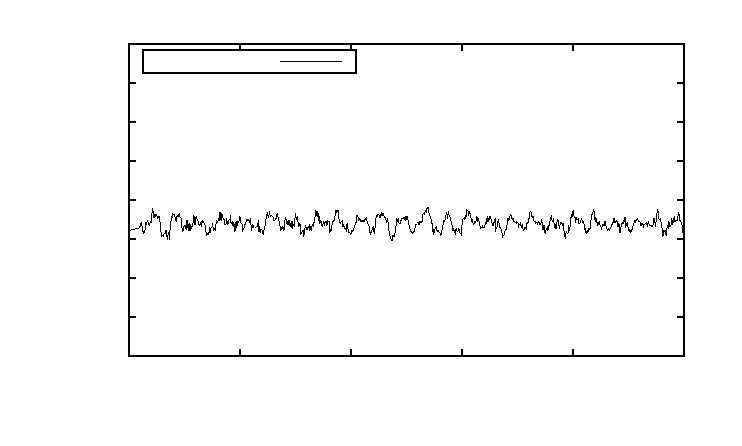
\includegraphics{schwebung-signal}}%
    \gplfronttext
  \end{picture}%
\endgroup

				\caption{}
				\label{fig:}
			\end{figure}
		
			\begin{figure}[htb]
				\centering
				% GNUPLOT: LaTeX picture with Postscript
\begingroup
  \makeatletter
  \providecommand\color[2][]{%
    \GenericError{(gnuplot) \space\space\space\@spaces}{%
      Package color not loaded in conjunction with
      terminal option `colourtext'%
    }{See the gnuplot documentation for explanation.%
    }{Either use 'blacktext' in gnuplot or load the package
      color.sty in LaTeX.}%
    \renewcommand\color[2][]{}%
  }%
  \providecommand\includegraphics[2][]{%
    \GenericError{(gnuplot) \space\space\space\@spaces}{%
      Package graphicx or graphics not loaded%
    }{See the gnuplot documentation for explanation.%
    }{The gnuplot epslatex terminal needs graphicx.sty or graphics.sty.}%
    \renewcommand\includegraphics[2][]{}%
  }%
  \providecommand\rotatebox[2]{#2}%
  \@ifundefined{ifGPcolor}{%
    \newif\ifGPcolor
    \GPcolorfalse
  }{}%
  \@ifundefined{ifGPblacktext}{%
    \newif\ifGPblacktext
    \GPblacktexttrue
  }{}%
  % define a \g@addto@macro without @ in the name:
  \let\gplgaddtomacro\g@addto@macro
  % define empty templates for all commands taking text:
  \gdef\gplbacktext{}%
  \gdef\gplfronttext{}%
  \makeatother
  \ifGPblacktext
    % no textcolor at all
    \def\colorrgb#1{}%
    \def\colorgray#1{}%
  \else
    % gray or color?
    \ifGPcolor
      \def\colorrgb#1{\color[rgb]{#1}}%
      \def\colorgray#1{\color[gray]{#1}}%
      \expandafter\def\csname LTw\endcsname{\color{white}}%
      \expandafter\def\csname LTb\endcsname{\color{black}}%
      \expandafter\def\csname LTa\endcsname{\color{black}}%
      \expandafter\def\csname LT0\endcsname{\color[rgb]{1,0,0}}%
      \expandafter\def\csname LT1\endcsname{\color[rgb]{0,1,0}}%
      \expandafter\def\csname LT2\endcsname{\color[rgb]{0,0,1}}%
      \expandafter\def\csname LT3\endcsname{\color[rgb]{1,0,1}}%
      \expandafter\def\csname LT4\endcsname{\color[rgb]{0,1,1}}%
      \expandafter\def\csname LT5\endcsname{\color[rgb]{1,1,0}}%
      \expandafter\def\csname LT6\endcsname{\color[rgb]{0,0,0}}%
      \expandafter\def\csname LT7\endcsname{\color[rgb]{1,0.3,0}}%
      \expandafter\def\csname LT8\endcsname{\color[rgb]{0.5,0.5,0.5}}%
    \else
      % gray
      \def\colorrgb#1{\color{black}}%
      \def\colorgray#1{\color[gray]{#1}}%
      \expandafter\def\csname LTw\endcsname{\color{white}}%
      \expandafter\def\csname LTb\endcsname{\color{black}}%
      \expandafter\def\csname LTa\endcsname{\color{black}}%
      \expandafter\def\csname LT0\endcsname{\color{black}}%
      \expandafter\def\csname LT1\endcsname{\color{black}}%
      \expandafter\def\csname LT2\endcsname{\color{black}}%
      \expandafter\def\csname LT3\endcsname{\color{black}}%
      \expandafter\def\csname LT4\endcsname{\color{black}}%
      \expandafter\def\csname LT5\endcsname{\color{black}}%
      \expandafter\def\csname LT6\endcsname{\color{black}}%
      \expandafter\def\csname LT7\endcsname{\color{black}}%
      \expandafter\def\csname LT8\endcsname{\color{black}}%
    \fi
  \fi
  \setlength{\unitlength}{0.0500bp}%
  \begin{picture}(6802.00,3968.00)%
    \gplgaddtomacro\gplbacktext{%
      \csname LTb\endcsname%
      \put(946,954){\makebox(0,0)[r]{\strut{} 0}}%
      \put(946,1454){\makebox(0,0)[r]{\strut{} 0.2}}%
      \put(946,1954){\makebox(0,0)[r]{\strut{} 0.4}}%
      \put(946,2453){\makebox(0,0)[r]{\strut{} 0.6}}%
      \put(946,2953){\makebox(0,0)[r]{\strut{} 0.8}}%
      \put(946,3453){\makebox(0,0)[r]{\strut{} 1}}%
      \put(1522,484){\makebox(0,0){\strut{} 496}}%
      \put(2410,484){\makebox(0,0){\strut{} 498}}%
      \put(3298,484){\makebox(0,0){\strut{} 500}}%
      \put(4185,484){\makebox(0,0){\strut{} 502}}%
      \put(5073,484){\makebox(0,0){\strut{} 504}}%
      \put(5961,484){\makebox(0,0){\strut{} 506}}%
      \put(176,2203){\rotatebox{-270}{\makebox(0,0){\strut{}Intensität}}}%
      \put(3741,154){\makebox(0,0){\strut{}Wellenlänge $\lambda \ [\unit{nm}]$}}%
    }%
    \gplgaddtomacro\gplfronttext{%
      \csname LTb\endcsname%
      \put(2398,3530){\makebox(0,0)[r]{\strut{}Messwerte}}%
    }%
    \gplbacktext
    \put(0,0){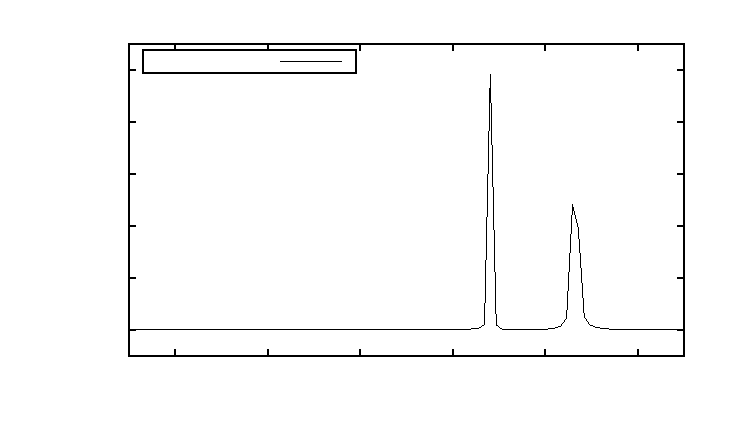
\includegraphics{schwebung-1}}%
    \gplfronttext
  \end{picture}%
\endgroup

				\caption{}
				\label{fig:schwebung-1}
			\end{figure}

			\begin{figure}[htb]
				\centering
				% GNUPLOT: LaTeX picture with Postscript
\begingroup
  \makeatletter
  \providecommand\color[2][]{%
    \GenericError{(gnuplot) \space\space\space\@spaces}{%
      Package color not loaded in conjunction with
      terminal option `colourtext'%
    }{See the gnuplot documentation for explanation.%
    }{Either use 'blacktext' in gnuplot or load the package
      color.sty in LaTeX.}%
    \renewcommand\color[2][]{}%
  }%
  \providecommand\includegraphics[2][]{%
    \GenericError{(gnuplot) \space\space\space\@spaces}{%
      Package graphicx or graphics not loaded%
    }{See the gnuplot documentation for explanation.%
    }{The gnuplot epslatex terminal needs graphicx.sty or graphics.sty.}%
    \renewcommand\includegraphics[2][]{}%
  }%
  \providecommand\rotatebox[2]{#2}%
  \@ifundefined{ifGPcolor}{%
    \newif\ifGPcolor
    \GPcolorfalse
  }{}%
  \@ifundefined{ifGPblacktext}{%
    \newif\ifGPblacktext
    \GPblacktexttrue
  }{}%
  % define a \g@addto@macro without @ in the name:
  \let\gplgaddtomacro\g@addto@macro
  % define empty templates for all commands taking text:
  \gdef\gplbacktext{}%
  \gdef\gplfronttext{}%
  \makeatother
  \ifGPblacktext
    % no textcolor at all
    \def\colorrgb#1{}%
    \def\colorgray#1{}%
  \else
    % gray or color?
    \ifGPcolor
      \def\colorrgb#1{\color[rgb]{#1}}%
      \def\colorgray#1{\color[gray]{#1}}%
      \expandafter\def\csname LTw\endcsname{\color{white}}%
      \expandafter\def\csname LTb\endcsname{\color{black}}%
      \expandafter\def\csname LTa\endcsname{\color{black}}%
      \expandafter\def\csname LT0\endcsname{\color[rgb]{1,0,0}}%
      \expandafter\def\csname LT1\endcsname{\color[rgb]{0,1,0}}%
      \expandafter\def\csname LT2\endcsname{\color[rgb]{0,0,1}}%
      \expandafter\def\csname LT3\endcsname{\color[rgb]{1,0,1}}%
      \expandafter\def\csname LT4\endcsname{\color[rgb]{0,1,1}}%
      \expandafter\def\csname LT5\endcsname{\color[rgb]{1,1,0}}%
      \expandafter\def\csname LT6\endcsname{\color[rgb]{0,0,0}}%
      \expandafter\def\csname LT7\endcsname{\color[rgb]{1,0.3,0}}%
      \expandafter\def\csname LT8\endcsname{\color[rgb]{0.5,0.5,0.5}}%
    \else
      % gray
      \def\colorrgb#1{\color{black}}%
      \def\colorgray#1{\color[gray]{#1}}%
      \expandafter\def\csname LTw\endcsname{\color{white}}%
      \expandafter\def\csname LTb\endcsname{\color{black}}%
      \expandafter\def\csname LTa\endcsname{\color{black}}%
      \expandafter\def\csname LT0\endcsname{\color{black}}%
      \expandafter\def\csname LT1\endcsname{\color{black}}%
      \expandafter\def\csname LT2\endcsname{\color{black}}%
      \expandafter\def\csname LT3\endcsname{\color{black}}%
      \expandafter\def\csname LT4\endcsname{\color{black}}%
      \expandafter\def\csname LT5\endcsname{\color{black}}%
      \expandafter\def\csname LT6\endcsname{\color{black}}%
      \expandafter\def\csname LT7\endcsname{\color{black}}%
      \expandafter\def\csname LT8\endcsname{\color{black}}%
    \fi
  \fi
  \setlength{\unitlength}{0.0500bp}%
  \begin{picture}(6802.00,3968.00)%
    \gplgaddtomacro\gplbacktext{%
      \csname LTb\endcsname%
      \put(946,954){\makebox(0,0)[r]{\strut{} 0}}%
      \put(946,1454){\makebox(0,0)[r]{\strut{} 0.2}}%
      \put(946,1954){\makebox(0,0)[r]{\strut{} 0.4}}%
      \put(946,2453){\makebox(0,0)[r]{\strut{} 0.6}}%
      \put(946,2953){\makebox(0,0)[r]{\strut{} 0.8}}%
      \put(946,3453){\makebox(0,0)[r]{\strut{} 1}}%
      \put(1562,484){\makebox(0,0){\strut{} 460}}%
      \put(2531,484){\makebox(0,0){\strut{} 480}}%
      \put(3499,484){\makebox(0,0){\strut{} 500}}%
      \put(4468,484){\makebox(0,0){\strut{} 520}}%
      \put(5436,484){\makebox(0,0){\strut{} 540}}%
      \put(6405,484){\makebox(0,0){\strut{} 560}}%
      \put(176,2203){\rotatebox{-270}{\makebox(0,0){\strut{}Intensität}}}%
      \put(3741,154){\makebox(0,0){\strut{}Wellenlänge $\lambda \ [\unit{nm}]$}}%
    }%
    \gplgaddtomacro\gplfronttext{%
      \csname LTb\endcsname%
      \put(2398,3530){\makebox(0,0)[r]{\strut{}Messwerte}}%
    }%
    \gplbacktext
    \put(0,0){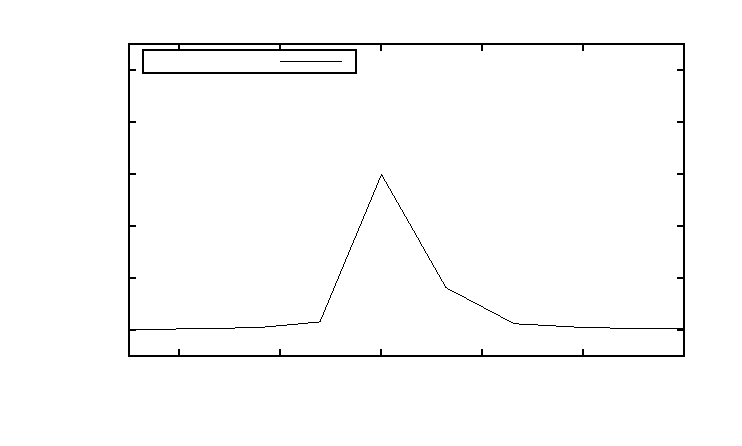
\includegraphics{schwebung-2}}%
    \gplfronttext
  \end{picture}%
\endgroup

				\caption{}
				\label{fig:schwebung-2}
			\end{figure}

			Die Abbildungen 789455 sieht man das Interferogramm 
		% subsubsection parameter_und_aufl_severm_gen (end)

		\subsubsection{Spektrum LED- und Gaslaser} % (fold)
		\label{ssub:spektrum_led_und_gaslaser}
		
			\begin{figure}[htb]
				\centering
				% GNUPLOT: LaTeX picture with Postscript
\begingroup
  \makeatletter
  \providecommand\color[2][]{%
    \GenericError{(gnuplot) \space\space\space\@spaces}{%
      Package color not loaded in conjunction with
      terminal option `colourtext'%
    }{See the gnuplot documentation for explanation.%
    }{Either use 'blacktext' in gnuplot or load the package
      color.sty in LaTeX.}%
    \renewcommand\color[2][]{}%
  }%
  \providecommand\includegraphics[2][]{%
    \GenericError{(gnuplot) \space\space\space\@spaces}{%
      Package graphicx or graphics not loaded%
    }{See the gnuplot documentation for explanation.%
    }{The gnuplot epslatex terminal needs graphicx.sty or graphics.sty.}%
    \renewcommand\includegraphics[2][]{}%
  }%
  \providecommand\rotatebox[2]{#2}%
  \@ifundefined{ifGPcolor}{%
    \newif\ifGPcolor
    \GPcolorfalse
  }{}%
  \@ifundefined{ifGPblacktext}{%
    \newif\ifGPblacktext
    \GPblacktexttrue
  }{}%
  % define a \g@addto@macro without @ in the name:
  \let\gplgaddtomacro\g@addto@macro
  % define empty templates for all commands taking text:
  \gdef\gplbacktext{}%
  \gdef\gplfronttext{}%
  \makeatother
  \ifGPblacktext
    % no textcolor at all
    \def\colorrgb#1{}%
    \def\colorgray#1{}%
  \else
    % gray or color?
    \ifGPcolor
      \def\colorrgb#1{\color[rgb]{#1}}%
      \def\colorgray#1{\color[gray]{#1}}%
      \expandafter\def\csname LTw\endcsname{\color{white}}%
      \expandafter\def\csname LTb\endcsname{\color{black}}%
      \expandafter\def\csname LTa\endcsname{\color{black}}%
      \expandafter\def\csname LT0\endcsname{\color[rgb]{1,0,0}}%
      \expandafter\def\csname LT1\endcsname{\color[rgb]{0,1,0}}%
      \expandafter\def\csname LT2\endcsname{\color[rgb]{0,0,1}}%
      \expandafter\def\csname LT3\endcsname{\color[rgb]{1,0,1}}%
      \expandafter\def\csname LT4\endcsname{\color[rgb]{0,1,1}}%
      \expandafter\def\csname LT5\endcsname{\color[rgb]{1,1,0}}%
      \expandafter\def\csname LT6\endcsname{\color[rgb]{0,0,0}}%
      \expandafter\def\csname LT7\endcsname{\color[rgb]{1,0.3,0}}%
      \expandafter\def\csname LT8\endcsname{\color[rgb]{0.5,0.5,0.5}}%
    \else
      % gray
      \def\colorrgb#1{\color{black}}%
      \def\colorgray#1{\color[gray]{#1}}%
      \expandafter\def\csname LTw\endcsname{\color{white}}%
      \expandafter\def\csname LTb\endcsname{\color{black}}%
      \expandafter\def\csname LTa\endcsname{\color{black}}%
      \expandafter\def\csname LT0\endcsname{\color{black}}%
      \expandafter\def\csname LT1\endcsname{\color{black}}%
      \expandafter\def\csname LT2\endcsname{\color{black}}%
      \expandafter\def\csname LT3\endcsname{\color{black}}%
      \expandafter\def\csname LT4\endcsname{\color{black}}%
      \expandafter\def\csname LT5\endcsname{\color{black}}%
      \expandafter\def\csname LT6\endcsname{\color{black}}%
      \expandafter\def\csname LT7\endcsname{\color{black}}%
      \expandafter\def\csname LT8\endcsname{\color{black}}%
    \fi
  \fi
  \setlength{\unitlength}{0.0500bp}%
  \begin{picture}(6802.00,3968.00)%
    \gplgaddtomacro\gplbacktext{%
      \csname LTb\endcsname%
      \put(946,1004){\makebox(0,0)[r]{\strut{} 0}}%
      \put(946,1604){\makebox(0,0)[r]{\strut{} 0.2}}%
      \put(946,2204){\makebox(0,0)[r]{\strut{} 0.4}}%
      \put(946,2803){\makebox(0,0)[r]{\strut{} 0.6}}%
      \put(946,3403){\makebox(0,0)[r]{\strut{} 0.8}}%
      \put(1078,484){\makebox(0,0){\strut{} 450}}%
      \put(2410,484){\makebox(0,0){\strut{} 500}}%
      \put(3742,484){\makebox(0,0){\strut{} 550}}%
      \put(5073,484){\makebox(0,0){\strut{} 600}}%
      \put(6405,484){\makebox(0,0){\strut{} 650}}%
      \put(176,2203){\rotatebox{-270}{\makebox(0,0){\strut{}Intensität}}}%
      \put(3741,154){\makebox(0,0){\strut{}Wellenlänge $\lambda \ [\unit{nm}]$}}%
    }%
    \gplgaddtomacro\gplfronttext{%
      \csname LTb\endcsname%
      \put(2398,3530){\makebox(0,0)[r]{\strut{}Messwerte}}%
    }%
    \gplbacktext
    \put(0,0){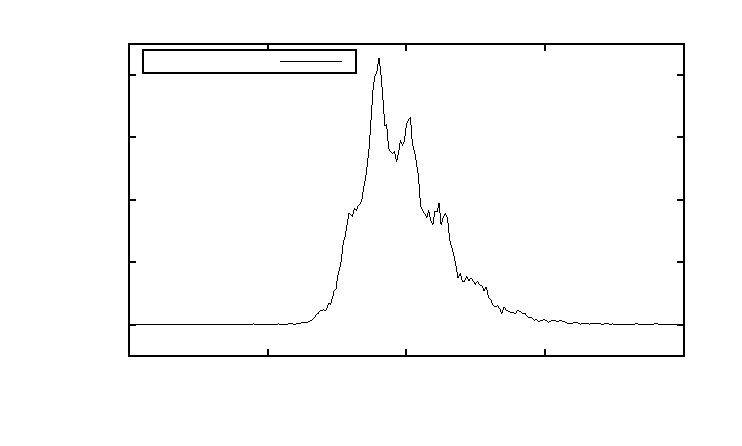
\includegraphics{led-spec}}%
    \gplfronttext
  \end{picture}%
\endgroup

				\caption{}
				\label{fig:}
			\end{figure}

			\begin{figure}[htb]
				\centering
				% GNUPLOT: LaTeX picture with Postscript
\begingroup
  \makeatletter
  \providecommand\color[2][]{%
    \GenericError{(gnuplot) \space\space\space\@spaces}{%
      Package color not loaded in conjunction with
      terminal option `colourtext'%
    }{See the gnuplot documentation for explanation.%
    }{Either use 'blacktext' in gnuplot or load the package
      color.sty in LaTeX.}%
    \renewcommand\color[2][]{}%
  }%
  \providecommand\includegraphics[2][]{%
    \GenericError{(gnuplot) \space\space\space\@spaces}{%
      Package graphicx or graphics not loaded%
    }{See the gnuplot documentation for explanation.%
    }{The gnuplot epslatex terminal needs graphicx.sty or graphics.sty.}%
    \renewcommand\includegraphics[2][]{}%
  }%
  \providecommand\rotatebox[2]{#2}%
  \@ifundefined{ifGPcolor}{%
    \newif\ifGPcolor
    \GPcolorfalse
  }{}%
  \@ifundefined{ifGPblacktext}{%
    \newif\ifGPblacktext
    \GPblacktexttrue
  }{}%
  % define a \g@addto@macro without @ in the name:
  \let\gplgaddtomacro\g@addto@macro
  % define empty templates for all commands taking text:
  \gdef\gplbacktext{}%
  \gdef\gplfronttext{}%
  \makeatother
  \ifGPblacktext
    % no textcolor at all
    \def\colorrgb#1{}%
    \def\colorgray#1{}%
  \else
    % gray or color?
    \ifGPcolor
      \def\colorrgb#1{\color[rgb]{#1}}%
      \def\colorgray#1{\color[gray]{#1}}%
      \expandafter\def\csname LTw\endcsname{\color{white}}%
      \expandafter\def\csname LTb\endcsname{\color{black}}%
      \expandafter\def\csname LTa\endcsname{\color{black}}%
      \expandafter\def\csname LT0\endcsname{\color[rgb]{1,0,0}}%
      \expandafter\def\csname LT1\endcsname{\color[rgb]{0,1,0}}%
      \expandafter\def\csname LT2\endcsname{\color[rgb]{0,0,1}}%
      \expandafter\def\csname LT3\endcsname{\color[rgb]{1,0,1}}%
      \expandafter\def\csname LT4\endcsname{\color[rgb]{0,1,1}}%
      \expandafter\def\csname LT5\endcsname{\color[rgb]{1,1,0}}%
      \expandafter\def\csname LT6\endcsname{\color[rgb]{0,0,0}}%
      \expandafter\def\csname LT7\endcsname{\color[rgb]{1,0.3,0}}%
      \expandafter\def\csname LT8\endcsname{\color[rgb]{0.5,0.5,0.5}}%
    \else
      % gray
      \def\colorrgb#1{\color{black}}%
      \def\colorgray#1{\color[gray]{#1}}%
      \expandafter\def\csname LTw\endcsname{\color{white}}%
      \expandafter\def\csname LTb\endcsname{\color{black}}%
      \expandafter\def\csname LTa\endcsname{\color{black}}%
      \expandafter\def\csname LT0\endcsname{\color{black}}%
      \expandafter\def\csname LT1\endcsname{\color{black}}%
      \expandafter\def\csname LT2\endcsname{\color{black}}%
      \expandafter\def\csname LT3\endcsname{\color{black}}%
      \expandafter\def\csname LT4\endcsname{\color{black}}%
      \expandafter\def\csname LT5\endcsname{\color{black}}%
      \expandafter\def\csname LT6\endcsname{\color{black}}%
      \expandafter\def\csname LT7\endcsname{\color{black}}%
      \expandafter\def\csname LT8\endcsname{\color{black}}%
    \fi
  \fi
  \setlength{\unitlength}{0.0500bp}%
  \begin{picture}(6802.00,3968.00)%
    \gplgaddtomacro\gplbacktext{%
      \csname LTb\endcsname%
      \put(946,847){\makebox(0,0)[r]{\strut{} 0}}%
      \put(946,1561){\makebox(0,0)[r]{\strut{} 0.5}}%
      \put(946,2275){\makebox(0,0)[r]{\strut{} 1}}%
      \put(946,2989){\makebox(0,0)[r]{\strut{} 1.5}}%
      \put(946,3703){\makebox(0,0)[r]{\strut{} 2}}%
      \put(1078,484){\makebox(0,0){\strut{} 650}}%
      \put(2143,484){\makebox(0,0){\strut{} 660}}%
      \put(3209,484){\makebox(0,0){\strut{} 670}}%
      \put(4274,484){\makebox(0,0){\strut{} 680}}%
      \put(5340,484){\makebox(0,0){\strut{} 690}}%
      \put(6405,484){\makebox(0,0){\strut{} 700}}%
      \put(176,2203){\rotatebox{-270}{\makebox(0,0){\strut{}Intensität}}}%
      \put(3741,154){\makebox(0,0){\strut{}Wellenlänge $\lambda \ [\unit{nm}]$}}%
    }%
    \gplgaddtomacro\gplfronttext{%
      \csname LTb\endcsname%
      \put(2398,3530){\makebox(0,0)[r]{\strut{}Messwerte}}%
    }%
    \gplbacktext
    \put(0,0){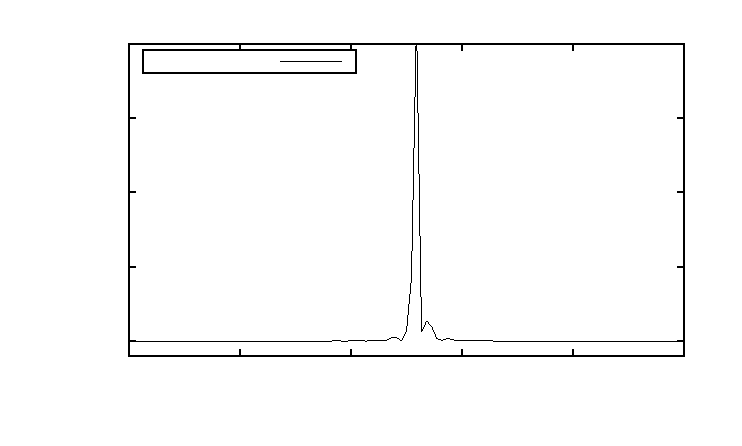
\includegraphics{led-laser-spec}}%
    \gplfronttext
  \end{picture}%
\endgroup

				\caption{}
				\label{fig:}
			\end{figure}

			\begin{figure}[htb]
				\centering
				% GNUPLOT: LaTeX picture with Postscript
\begingroup
  \makeatletter
  \providecommand\color[2][]{%
    \GenericError{(gnuplot) \space\space\space\@spaces}{%
      Package color not loaded in conjunction with
      terminal option `colourtext'%
    }{See the gnuplot documentation for explanation.%
    }{Either use 'blacktext' in gnuplot or load the package
      color.sty in LaTeX.}%
    \renewcommand\color[2][]{}%
  }%
  \providecommand\includegraphics[2][]{%
    \GenericError{(gnuplot) \space\space\space\@spaces}{%
      Package graphicx or graphics not loaded%
    }{See the gnuplot documentation for explanation.%
    }{The gnuplot epslatex terminal needs graphicx.sty or graphics.sty.}%
    \renewcommand\includegraphics[2][]{}%
  }%
  \providecommand\rotatebox[2]{#2}%
  \@ifundefined{ifGPcolor}{%
    \newif\ifGPcolor
    \GPcolorfalse
  }{}%
  \@ifundefined{ifGPblacktext}{%
    \newif\ifGPblacktext
    \GPblacktexttrue
  }{}%
  % define a \g@addto@macro without @ in the name:
  \let\gplgaddtomacro\g@addto@macro
  % define empty templates for all commands taking text:
  \gdef\gplbacktext{}%
  \gdef\gplfronttext{}%
  \makeatother
  \ifGPblacktext
    % no textcolor at all
    \def\colorrgb#1{}%
    \def\colorgray#1{}%
  \else
    % gray or color?
    \ifGPcolor
      \def\colorrgb#1{\color[rgb]{#1}}%
      \def\colorgray#1{\color[gray]{#1}}%
      \expandafter\def\csname LTw\endcsname{\color{white}}%
      \expandafter\def\csname LTb\endcsname{\color{black}}%
      \expandafter\def\csname LTa\endcsname{\color{black}}%
      \expandafter\def\csname LT0\endcsname{\color[rgb]{1,0,0}}%
      \expandafter\def\csname LT1\endcsname{\color[rgb]{0,1,0}}%
      \expandafter\def\csname LT2\endcsname{\color[rgb]{0,0,1}}%
      \expandafter\def\csname LT3\endcsname{\color[rgb]{1,0,1}}%
      \expandafter\def\csname LT4\endcsname{\color[rgb]{0,1,1}}%
      \expandafter\def\csname LT5\endcsname{\color[rgb]{1,1,0}}%
      \expandafter\def\csname LT6\endcsname{\color[rgb]{0,0,0}}%
      \expandafter\def\csname LT7\endcsname{\color[rgb]{1,0.3,0}}%
      \expandafter\def\csname LT8\endcsname{\color[rgb]{0.5,0.5,0.5}}%
    \else
      % gray
      \def\colorrgb#1{\color{black}}%
      \def\colorgray#1{\color[gray]{#1}}%
      \expandafter\def\csname LTw\endcsname{\color{white}}%
      \expandafter\def\csname LTb\endcsname{\color{black}}%
      \expandafter\def\csname LTa\endcsname{\color{black}}%
      \expandafter\def\csname LT0\endcsname{\color{black}}%
      \expandafter\def\csname LT1\endcsname{\color{black}}%
      \expandafter\def\csname LT2\endcsname{\color{black}}%
      \expandafter\def\csname LT3\endcsname{\color{black}}%
      \expandafter\def\csname LT4\endcsname{\color{black}}%
      \expandafter\def\csname LT5\endcsname{\color{black}}%
      \expandafter\def\csname LT6\endcsname{\color{black}}%
      \expandafter\def\csname LT7\endcsname{\color{black}}%
      \expandafter\def\csname LT8\endcsname{\color{black}}%
    \fi
  \fi
  \setlength{\unitlength}{0.0500bp}%
  \begin{picture}(6802.00,3968.00)%
    \gplgaddtomacro\gplbacktext{%
      \csname LTb\endcsname%
      \put(946,801){\makebox(0,0)[r]{\strut{} 0}}%
      \put(946,1284){\makebox(0,0)[r]{\strut{} 0.5}}%
      \put(946,1768){\makebox(0,0)[r]{\strut{} 1}}%
      \put(946,2252){\makebox(0,0)[r]{\strut{} 1.5}}%
      \put(946,2736){\makebox(0,0)[r]{\strut{} 2}}%
      \put(946,3219){\makebox(0,0)[r]{\strut{} 2.5}}%
      \put(946,3703){\makebox(0,0)[r]{\strut{} 3}}%
      \put(1078,484){\makebox(0,0){\strut{} 520}}%
      \put(2410,484){\makebox(0,0){\strut{} 525}}%
      \put(3742,484){\makebox(0,0){\strut{} 530}}%
      \put(5073,484){\makebox(0,0){\strut{} 535}}%
      \put(6405,484){\makebox(0,0){\strut{} 540}}%
      \put(176,2203){\rotatebox{-270}{\makebox(0,0){\strut{}Intensität}}}%
      \put(3741,154){\makebox(0,0){\strut{}Wellenlänge $\lambda \ [\unit{nm}]$}}%
    }%
    \gplgaddtomacro\gplfronttext{%
      \csname LTb\endcsname%
      \put(2398,3530){\makebox(0,0)[r]{\strut{}Messwerte}}%
    }%
    \gplbacktext
    \put(0,0){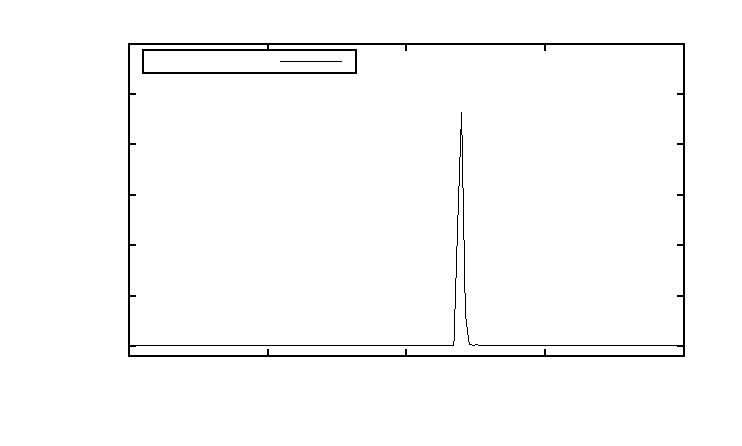
\includegraphics{g-laser-spec}}%
    \gplfronttext
  \end{picture}%
\endgroup

				\caption{}
				\label{fig:}
			\end{figure}

		% subsubsection spektrum_led_und_gaslaser (end)

		\subsubsection{Spektrum Natrium- und Quecksilberdampflampe} % (fold)
		\label{ssub:spektrum_natrium_und_quecksilberdampflampe}

			\begin{figure}[htb]
				\centering
				% GNUPLOT: LaTeX picture with Postscript
\begingroup
  \makeatletter
  \providecommand\color[2][]{%
    \GenericError{(gnuplot) \space\space\space\@spaces}{%
      Package color not loaded in conjunction with
      terminal option `colourtext'%
    }{See the gnuplot documentation for explanation.%
    }{Either use 'blacktext' in gnuplot or load the package
      color.sty in LaTeX.}%
    \renewcommand\color[2][]{}%
  }%
  \providecommand\includegraphics[2][]{%
    \GenericError{(gnuplot) \space\space\space\@spaces}{%
      Package graphicx or graphics not loaded%
    }{See the gnuplot documentation for explanation.%
    }{The gnuplot epslatex terminal needs graphicx.sty or graphics.sty.}%
    \renewcommand\includegraphics[2][]{}%
  }%
  \providecommand\rotatebox[2]{#2}%
  \@ifundefined{ifGPcolor}{%
    \newif\ifGPcolor
    \GPcolorfalse
  }{}%
  \@ifundefined{ifGPblacktext}{%
    \newif\ifGPblacktext
    \GPblacktexttrue
  }{}%
  % define a \g@addto@macro without @ in the name:
  \let\gplgaddtomacro\g@addto@macro
  % define empty templates for all commands taking text:
  \gdef\gplbacktext{}%
  \gdef\gplfronttext{}%
  \makeatother
  \ifGPblacktext
    % no textcolor at all
    \def\colorrgb#1{}%
    \def\colorgray#1{}%
  \else
    % gray or color?
    \ifGPcolor
      \def\colorrgb#1{\color[rgb]{#1}}%
      \def\colorgray#1{\color[gray]{#1}}%
      \expandafter\def\csname LTw\endcsname{\color{white}}%
      \expandafter\def\csname LTb\endcsname{\color{black}}%
      \expandafter\def\csname LTa\endcsname{\color{black}}%
      \expandafter\def\csname LT0\endcsname{\color[rgb]{1,0,0}}%
      \expandafter\def\csname LT1\endcsname{\color[rgb]{0,1,0}}%
      \expandafter\def\csname LT2\endcsname{\color[rgb]{0,0,1}}%
      \expandafter\def\csname LT3\endcsname{\color[rgb]{1,0,1}}%
      \expandafter\def\csname LT4\endcsname{\color[rgb]{0,1,1}}%
      \expandafter\def\csname LT5\endcsname{\color[rgb]{1,1,0}}%
      \expandafter\def\csname LT6\endcsname{\color[rgb]{0,0,0}}%
      \expandafter\def\csname LT7\endcsname{\color[rgb]{1,0.3,0}}%
      \expandafter\def\csname LT8\endcsname{\color[rgb]{0.5,0.5,0.5}}%
    \else
      % gray
      \def\colorrgb#1{\color{black}}%
      \def\colorgray#1{\color[gray]{#1}}%
      \expandafter\def\csname LTw\endcsname{\color{white}}%
      \expandafter\def\csname LTb\endcsname{\color{black}}%
      \expandafter\def\csname LTa\endcsname{\color{black}}%
      \expandafter\def\csname LT0\endcsname{\color{black}}%
      \expandafter\def\csname LT1\endcsname{\color{black}}%
      \expandafter\def\csname LT2\endcsname{\color{black}}%
      \expandafter\def\csname LT3\endcsname{\color{black}}%
      \expandafter\def\csname LT4\endcsname{\color{black}}%
      \expandafter\def\csname LT5\endcsname{\color{black}}%
      \expandafter\def\csname LT6\endcsname{\color{black}}%
      \expandafter\def\csname LT7\endcsname{\color{black}}%
      \expandafter\def\csname LT8\endcsname{\color{black}}%
    \fi
  \fi
  \setlength{\unitlength}{0.0500bp}%
  \begin{picture}(6802.00,3968.00)%
    \gplgaddtomacro\gplbacktext{%
      \csname LTb\endcsname%
      \put(814,724){\makebox(0,0)[r]{\strut{} 0}}%
      \put(814,1121){\makebox(0,0)[r]{\strut{} 2}}%
      \put(814,1518){\makebox(0,0)[r]{\strut{} 4}}%
      \put(814,1916){\makebox(0,0)[r]{\strut{} 6}}%
      \put(814,2313){\makebox(0,0)[r]{\strut{} 8}}%
      \put(814,2710){\makebox(0,0)[r]{\strut{} 10}}%
      \put(814,3107){\makebox(0,0)[r]{\strut{} 12}}%
      \put(814,3504){\makebox(0,0)[r]{\strut{} 14}}%
      \put(946,484){\makebox(0,0){\strut{} 585}}%
      \put(1726,484){\makebox(0,0){\strut{} 586}}%
      \put(2506,484){\makebox(0,0){\strut{} 587}}%
      \put(3286,484){\makebox(0,0){\strut{} 588}}%
      \put(4065,484){\makebox(0,0){\strut{} 589}}%
      \put(4845,484){\makebox(0,0){\strut{} 590}}%
      \put(5625,484){\makebox(0,0){\strut{} 591}}%
      \put(6405,484){\makebox(0,0){\strut{} 592}}%
      \put(176,2203){\rotatebox{-270}{\makebox(0,0){\strut{}Intensität}}}%
      \put(3675,154){\makebox(0,0){\strut{}Wellenlänge $\lambda \ [\unit{nm}]$}}%
    }%
    \gplgaddtomacro\gplfronttext{%
      \csname LTb\endcsname%
      \put(2266,3530){\makebox(0,0)[r]{\strut{}Messwerte}}%
    }%
    \gplbacktext
    \put(0,0){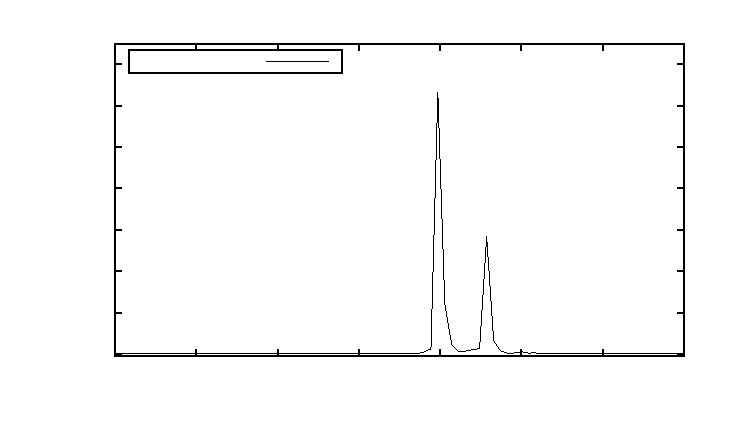
\includegraphics{na-dd}}%
    \gplfronttext
  \end{picture}%
\endgroup

				\caption{}
				\label{fig:}
			\end{figure}

			\begin{figure}[htb]
				\centering
				% GNUPLOT: LaTeX picture with Postscript
\begingroup
  \makeatletter
  \providecommand\color[2][]{%
    \GenericError{(gnuplot) \space\space\space\@spaces}{%
      Package color not loaded in conjunction with
      terminal option `colourtext'%
    }{See the gnuplot documentation for explanation.%
    }{Either use 'blacktext' in gnuplot or load the package
      color.sty in LaTeX.}%
    \renewcommand\color[2][]{}%
  }%
  \providecommand\includegraphics[2][]{%
    \GenericError{(gnuplot) \space\space\space\@spaces}{%
      Package graphicx or graphics not loaded%
    }{See the gnuplot documentation for explanation.%
    }{The gnuplot epslatex terminal needs graphicx.sty or graphics.sty.}%
    \renewcommand\includegraphics[2][]{}%
  }%
  \providecommand\rotatebox[2]{#2}%
  \@ifundefined{ifGPcolor}{%
    \newif\ifGPcolor
    \GPcolorfalse
  }{}%
  \@ifundefined{ifGPblacktext}{%
    \newif\ifGPblacktext
    \GPblacktexttrue
  }{}%
  % define a \g@addto@macro without @ in the name:
  \let\gplgaddtomacro\g@addto@macro
  % define empty templates for all commands taking text:
  \gdef\gplbacktext{}%
  \gdef\gplfronttext{}%
  \makeatother
  \ifGPblacktext
    % no textcolor at all
    \def\colorrgb#1{}%
    \def\colorgray#1{}%
  \else
    % gray or color?
    \ifGPcolor
      \def\colorrgb#1{\color[rgb]{#1}}%
      \def\colorgray#1{\color[gray]{#1}}%
      \expandafter\def\csname LTw\endcsname{\color{white}}%
      \expandafter\def\csname LTb\endcsname{\color{black}}%
      \expandafter\def\csname LTa\endcsname{\color{black}}%
      \expandafter\def\csname LT0\endcsname{\color[rgb]{1,0,0}}%
      \expandafter\def\csname LT1\endcsname{\color[rgb]{0,1,0}}%
      \expandafter\def\csname LT2\endcsname{\color[rgb]{0,0,1}}%
      \expandafter\def\csname LT3\endcsname{\color[rgb]{1,0,1}}%
      \expandafter\def\csname LT4\endcsname{\color[rgb]{0,1,1}}%
      \expandafter\def\csname LT5\endcsname{\color[rgb]{1,1,0}}%
      \expandafter\def\csname LT6\endcsname{\color[rgb]{0,0,0}}%
      \expandafter\def\csname LT7\endcsname{\color[rgb]{1,0.3,0}}%
      \expandafter\def\csname LT8\endcsname{\color[rgb]{0.5,0.5,0.5}}%
    \else
      % gray
      \def\colorrgb#1{\color{black}}%
      \def\colorgray#1{\color[gray]{#1}}%
      \expandafter\def\csname LTw\endcsname{\color{white}}%
      \expandafter\def\csname LTb\endcsname{\color{black}}%
      \expandafter\def\csname LTa\endcsname{\color{black}}%
      \expandafter\def\csname LT0\endcsname{\color{black}}%
      \expandafter\def\csname LT1\endcsname{\color{black}}%
      \expandafter\def\csname LT2\endcsname{\color{black}}%
      \expandafter\def\csname LT3\endcsname{\color{black}}%
      \expandafter\def\csname LT4\endcsname{\color{black}}%
      \expandafter\def\csname LT5\endcsname{\color{black}}%
      \expandafter\def\csname LT6\endcsname{\color{black}}%
      \expandafter\def\csname LT7\endcsname{\color{black}}%
      \expandafter\def\csname LT8\endcsname{\color{black}}%
    \fi
  \fi
  \setlength{\unitlength}{0.0500bp}%
  \begin{picture}(6802.00,3968.00)%
    \gplgaddtomacro\gplbacktext{%
      \csname LTb\endcsname%
      \put(682,763){\makebox(0,0)[r]{\strut{} 0}}%
      \put(682,1351){\makebox(0,0)[r]{\strut{} 1}}%
      \put(682,1939){\makebox(0,0)[r]{\strut{} 2}}%
      \put(682,2527){\makebox(0,0)[r]{\strut{} 3}}%
      \put(682,3115){\makebox(0,0)[r]{\strut{} 4}}%
      \put(682,3703){\makebox(0,0)[r]{\strut{} 5}}%
      \put(1322,484){\makebox(0,0){\strut{} 400}}%
      \put(2593,484){\makebox(0,0){\strut{} 450}}%
      \put(3864,484){\makebox(0,0){\strut{} 500}}%
      \put(5134,484){\makebox(0,0){\strut{} 550}}%
      \put(6405,484){\makebox(0,0){\strut{} 600}}%
      \put(176,2203){\rotatebox{-270}{\makebox(0,0){\strut{}Intensität}}}%
      \put(3609,154){\makebox(0,0){\strut{}Wellenlänge $\lambda \ [\unit{nm}]$}}%
    }%
    \gplgaddtomacro\gplfronttext{%
      \csname LTb\endcsname%
      \put(3776,3530){\makebox(0,0)[r]{\strut{}Messwerte}}%
    }%
    \gplbacktext
    \put(0,0){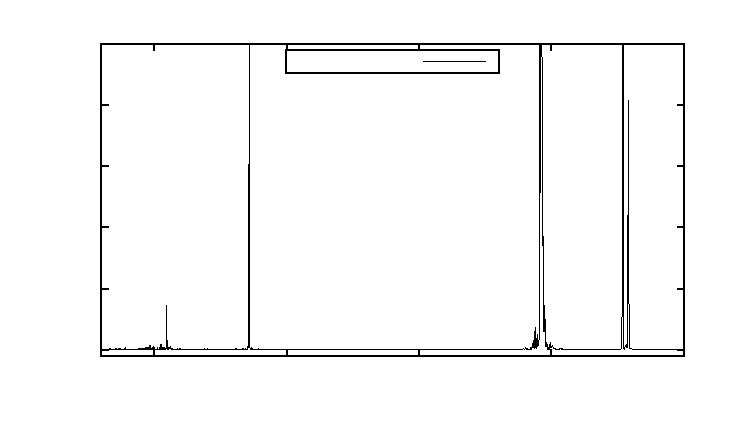
\includegraphics{hg-spec}}%
    \gplfronttext
  \end{picture}%
\endgroup

				\caption{}
				\label{fig:}
			\end{figure}
			
		% subsubsection spektrum_natrium_und_quecksilberdampflampe (end)


		\subsubsection{Glühlampenspektrum und Detektorbandlücke} % (fold)
		\label{ssub:gl_hlampenspektrum}

			\begin{figure}[htb]
				\centering
				% GNUPLOT: LaTeX picture with Postscript
\begingroup
  \makeatletter
  \providecommand\color[2][]{%
    \GenericError{(gnuplot) \space\space\space\@spaces}{%
      Package color not loaded in conjunction with
      terminal option `colourtext'%
    }{See the gnuplot documentation for explanation.%
    }{Either use 'blacktext' in gnuplot or load the package
      color.sty in LaTeX.}%
    \renewcommand\color[2][]{}%
  }%
  \providecommand\includegraphics[2][]{%
    \GenericError{(gnuplot) \space\space\space\@spaces}{%
      Package graphicx or graphics not loaded%
    }{See the gnuplot documentation for explanation.%
    }{The gnuplot epslatex terminal needs graphicx.sty or graphics.sty.}%
    \renewcommand\includegraphics[2][]{}%
  }%
  \providecommand\rotatebox[2]{#2}%
  \@ifundefined{ifGPcolor}{%
    \newif\ifGPcolor
    \GPcolorfalse
  }{}%
  \@ifundefined{ifGPblacktext}{%
    \newif\ifGPblacktext
    \GPblacktexttrue
  }{}%
  % define a \g@addto@macro without @ in the name:
  \let\gplgaddtomacro\g@addto@macro
  % define empty templates for all commands taking text:
  \gdef\gplbacktext{}%
  \gdef\gplfronttext{}%
  \makeatother
  \ifGPblacktext
    % no textcolor at all
    \def\colorrgb#1{}%
    \def\colorgray#1{}%
  \else
    % gray or color?
    \ifGPcolor
      \def\colorrgb#1{\color[rgb]{#1}}%
      \def\colorgray#1{\color[gray]{#1}}%
      \expandafter\def\csname LTw\endcsname{\color{white}}%
      \expandafter\def\csname LTb\endcsname{\color{black}}%
      \expandafter\def\csname LTa\endcsname{\color{black}}%
      \expandafter\def\csname LT0\endcsname{\color[rgb]{1,0,0}}%
      \expandafter\def\csname LT1\endcsname{\color[rgb]{0,1,0}}%
      \expandafter\def\csname LT2\endcsname{\color[rgb]{0,0,1}}%
      \expandafter\def\csname LT3\endcsname{\color[rgb]{1,0,1}}%
      \expandafter\def\csname LT4\endcsname{\color[rgb]{0,1,1}}%
      \expandafter\def\csname LT5\endcsname{\color[rgb]{1,1,0}}%
      \expandafter\def\csname LT6\endcsname{\color[rgb]{0,0,0}}%
      \expandafter\def\csname LT7\endcsname{\color[rgb]{1,0.3,0}}%
      \expandafter\def\csname LT8\endcsname{\color[rgb]{0.5,0.5,0.5}}%
    \else
      % gray
      \def\colorrgb#1{\color{black}}%
      \def\colorgray#1{\color[gray]{#1}}%
      \expandafter\def\csname LTw\endcsname{\color{white}}%
      \expandafter\def\csname LTb\endcsname{\color{black}}%
      \expandafter\def\csname LTa\endcsname{\color{black}}%
      \expandafter\def\csname LT0\endcsname{\color{black}}%
      \expandafter\def\csname LT1\endcsname{\color{black}}%
      \expandafter\def\csname LT2\endcsname{\color{black}}%
      \expandafter\def\csname LT3\endcsname{\color{black}}%
      \expandafter\def\csname LT4\endcsname{\color{black}}%
      \expandafter\def\csname LT5\endcsname{\color{black}}%
      \expandafter\def\csname LT6\endcsname{\color{black}}%
      \expandafter\def\csname LT7\endcsname{\color{black}}%
      \expandafter\def\csname LT8\endcsname{\color{black}}%
    \fi
  \fi
  \setlength{\unitlength}{0.0500bp}%
  \begin{picture}(6802.00,3968.00)%
    \gplgaddtomacro\gplbacktext{%
      \csname LTb\endcsname%
      \put(946,954){\makebox(0,0)[r]{\strut{} 0}}%
      \put(946,1454){\makebox(0,0)[r]{\strut{} 0.2}}%
      \put(946,1954){\makebox(0,0)[r]{\strut{} 0.4}}%
      \put(946,2453){\makebox(0,0)[r]{\strut{} 0.6}}%
      \put(946,2953){\makebox(0,0)[r]{\strut{} 0.8}}%
      \put(946,3453){\makebox(0,0)[r]{\strut{} 1}}%
      \put(1078,484){\makebox(0,0){\strut{} 400}}%
      \put(1744,484){\makebox(0,0){\strut{} 500}}%
      \put(2410,484){\makebox(0,0){\strut{} 600}}%
      \put(3076,484){\makebox(0,0){\strut{} 700}}%
      \put(3742,484){\makebox(0,0){\strut{} 800}}%
      \put(4407,484){\makebox(0,0){\strut{} 900}}%
      \put(5073,484){\makebox(0,0){\strut{} 1000}}%
      \put(5739,484){\makebox(0,0){\strut{} 1100}}%
      \put(6405,484){\makebox(0,0){\strut{} 1200}}%
      \put(176,2203){\rotatebox{-270}{\makebox(0,0){\strut{}Intensität}}}%
      \put(3741,154){\makebox(0,0){\strut{}Wellenlänge $\lambda \ [\unit{nm}]$}}%
    }%
    \gplgaddtomacro\gplfronttext{%
      \csname LTb\endcsname%
      \put(2398,3530){\makebox(0,0)[r]{\strut{}Messwerte}}%
    }%
    \gplbacktext
    \put(0,0){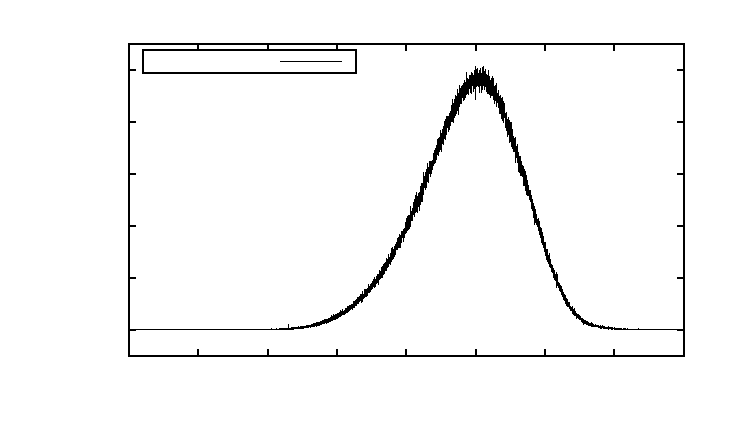
\includegraphics{lamp-spec}}%
    \gplfronttext
  \end{picture}%
\endgroup

				\caption{}
				\label{fig:}
			\end{figure}

			\begin{figure}[htb]
				\centering
				% GNUPLOT: LaTeX picture with Postscript
\begingroup
  \makeatletter
  \providecommand\color[2][]{%
    \GenericError{(gnuplot) \space\space\space\@spaces}{%
      Package color not loaded in conjunction with
      terminal option `colourtext'%
    }{See the gnuplot documentation for explanation.%
    }{Either use 'blacktext' in gnuplot or load the package
      color.sty in LaTeX.}%
    \renewcommand\color[2][]{}%
  }%
  \providecommand\includegraphics[2][]{%
    \GenericError{(gnuplot) \space\space\space\@spaces}{%
      Package graphicx or graphics not loaded%
    }{See the gnuplot documentation for explanation.%
    }{The gnuplot epslatex terminal needs graphicx.sty or graphics.sty.}%
    \renewcommand\includegraphics[2][]{}%
  }%
  \providecommand\rotatebox[2]{#2}%
  \@ifundefined{ifGPcolor}{%
    \newif\ifGPcolor
    \GPcolorfalse
  }{}%
  \@ifundefined{ifGPblacktext}{%
    \newif\ifGPblacktext
    \GPblacktexttrue
  }{}%
  % define a \g@addto@macro without @ in the name:
  \let\gplgaddtomacro\g@addto@macro
  % define empty templates for all commands taking text:
  \gdef\gplbacktext{}%
  \gdef\gplfronttext{}%
  \makeatother
  \ifGPblacktext
    % no textcolor at all
    \def\colorrgb#1{}%
    \def\colorgray#1{}%
  \else
    % gray or color?
    \ifGPcolor
      \def\colorrgb#1{\color[rgb]{#1}}%
      \def\colorgray#1{\color[gray]{#1}}%
      \expandafter\def\csname LTw\endcsname{\color{white}}%
      \expandafter\def\csname LTb\endcsname{\color{black}}%
      \expandafter\def\csname LTa\endcsname{\color{black}}%
      \expandafter\def\csname LT0\endcsname{\color[rgb]{1,0,0}}%
      \expandafter\def\csname LT1\endcsname{\color[rgb]{0,1,0}}%
      \expandafter\def\csname LT2\endcsname{\color[rgb]{0,0,1}}%
      \expandafter\def\csname LT3\endcsname{\color[rgb]{1,0,1}}%
      \expandafter\def\csname LT4\endcsname{\color[rgb]{0,1,1}}%
      \expandafter\def\csname LT5\endcsname{\color[rgb]{1,1,0}}%
      \expandafter\def\csname LT6\endcsname{\color[rgb]{0,0,0}}%
      \expandafter\def\csname LT7\endcsname{\color[rgb]{1,0.3,0}}%
      \expandafter\def\csname LT8\endcsname{\color[rgb]{0.5,0.5,0.5}}%
    \else
      % gray
      \def\colorrgb#1{\color{black}}%
      \def\colorgray#1{\color[gray]{#1}}%
      \expandafter\def\csname LTw\endcsname{\color{white}}%
      \expandafter\def\csname LTb\endcsname{\color{black}}%
      \expandafter\def\csname LTa\endcsname{\color{black}}%
      \expandafter\def\csname LT0\endcsname{\color{black}}%
      \expandafter\def\csname LT1\endcsname{\color{black}}%
      \expandafter\def\csname LT2\endcsname{\color{black}}%
      \expandafter\def\csname LT3\endcsname{\color{black}}%
      \expandafter\def\csname LT4\endcsname{\color{black}}%
      \expandafter\def\csname LT5\endcsname{\color{black}}%
      \expandafter\def\csname LT6\endcsname{\color{black}}%
      \expandafter\def\csname LT7\endcsname{\color{black}}%
      \expandafter\def\csname LT8\endcsname{\color{black}}%
    \fi
  \fi
  \setlength{\unitlength}{0.0500bp}%
  \begin{picture}(6802.00,3968.00)%
    \gplgaddtomacro\gplbacktext{%
      \csname LTb\endcsname%
      \put(946,954){\makebox(0,0)[r]{\strut{} 0}}%
      \put(946,1454){\makebox(0,0)[r]{\strut{} 0.2}}%
      \put(946,1954){\makebox(0,0)[r]{\strut{} 0.4}}%
      \put(946,2453){\makebox(0,0)[r]{\strut{} 0.6}}%
      \put(946,2953){\makebox(0,0)[r]{\strut{} 0.8}}%
      \put(946,3453){\makebox(0,0)[r]{\strut{} 1}}%
      \put(1283,484){\makebox(0,0){\strut{} 500}}%
      \put(2307,484){\makebox(0,0){\strut{} 1000}}%
      \put(3332,484){\makebox(0,0){\strut{} 1500}}%
      \put(4356,484){\makebox(0,0){\strut{} 2000}}%
      \put(5381,484){\makebox(0,0){\strut{} 2500}}%
      \put(6405,484){\makebox(0,0){\strut{} 3000}}%
      \put(176,2203){\rotatebox{-270}{\makebox(0,0){\strut{}Intensität}}}%
      \put(3741,154){\makebox(0,0){\strut{}Wellenlänge $\lambda \ [\unit{nm}]$}}%
    }%
    \gplgaddtomacro\gplfronttext{%
      \csname LTb\endcsname%
      \put(2398,3530){\makebox(0,0)[r]{\strut{}Messwerte}}%
    }%
    \gplbacktext
    \put(0,0){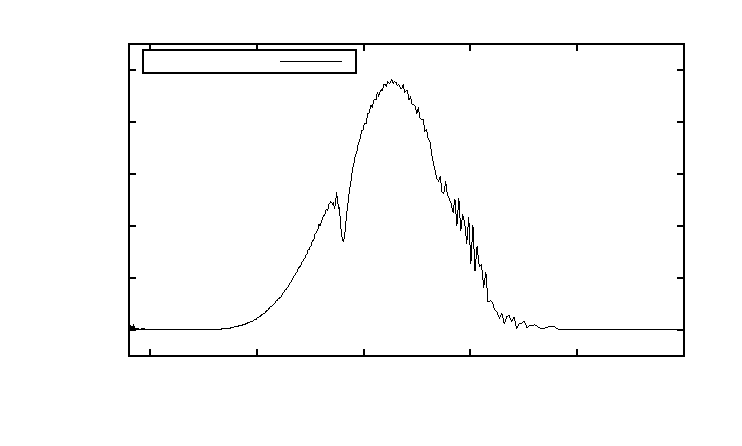
\includegraphics{lamp-pbse-spec}}%
    \gplfronttext
  \end{picture}%
\endgroup

				\caption{}
				\label{fig:}
			\end{figure}

			\begin{figure}[htb]
				\centering
				% GNUPLOT: LaTeX picture with Postscript
\begingroup
  \makeatletter
  \providecommand\color[2][]{%
    \GenericError{(gnuplot) \space\space\space\@spaces}{%
      Package color not loaded in conjunction with
      terminal option `colourtext'%
    }{See the gnuplot documentation for explanation.%
    }{Either use 'blacktext' in gnuplot or load the package
      color.sty in LaTeX.}%
    \renewcommand\color[2][]{}%
  }%
  \providecommand\includegraphics[2][]{%
    \GenericError{(gnuplot) \space\space\space\@spaces}{%
      Package graphicx or graphics not loaded%
    }{See the gnuplot documentation for explanation.%
    }{The gnuplot epslatex terminal needs graphicx.sty or graphics.sty.}%
    \renewcommand\includegraphics[2][]{}%
  }%
  \providecommand\rotatebox[2]{#2}%
  \@ifundefined{ifGPcolor}{%
    \newif\ifGPcolor
    \GPcolorfalse
  }{}%
  \@ifundefined{ifGPblacktext}{%
    \newif\ifGPblacktext
    \GPblacktexttrue
  }{}%
  % define a \g@addto@macro without @ in the name:
  \let\gplgaddtomacro\g@addto@macro
  % define empty templates for all commands taking text:
  \gdef\gplbacktext{}%
  \gdef\gplfronttext{}%
  \makeatother
  \ifGPblacktext
    % no textcolor at all
    \def\colorrgb#1{}%
    \def\colorgray#1{}%
  \else
    % gray or color?
    \ifGPcolor
      \def\colorrgb#1{\color[rgb]{#1}}%
      \def\colorgray#1{\color[gray]{#1}}%
      \expandafter\def\csname LTw\endcsname{\color{white}}%
      \expandafter\def\csname LTb\endcsname{\color{black}}%
      \expandafter\def\csname LTa\endcsname{\color{black}}%
      \expandafter\def\csname LT0\endcsname{\color[rgb]{1,0,0}}%
      \expandafter\def\csname LT1\endcsname{\color[rgb]{0,1,0}}%
      \expandafter\def\csname LT2\endcsname{\color[rgb]{0,0,1}}%
      \expandafter\def\csname LT3\endcsname{\color[rgb]{1,0,1}}%
      \expandafter\def\csname LT4\endcsname{\color[rgb]{0,1,1}}%
      \expandafter\def\csname LT5\endcsname{\color[rgb]{1,1,0}}%
      \expandafter\def\csname LT6\endcsname{\color[rgb]{0,0,0}}%
      \expandafter\def\csname LT7\endcsname{\color[rgb]{1,0.3,0}}%
      \expandafter\def\csname LT8\endcsname{\color[rgb]{0.5,0.5,0.5}}%
    \else
      % gray
      \def\colorrgb#1{\color{black}}%
      \def\colorgray#1{\color[gray]{#1}}%
      \expandafter\def\csname LTw\endcsname{\color{white}}%
      \expandafter\def\csname LTb\endcsname{\color{black}}%
      \expandafter\def\csname LTa\endcsname{\color{black}}%
      \expandafter\def\csname LT0\endcsname{\color{black}}%
      \expandafter\def\csname LT1\endcsname{\color{black}}%
      \expandafter\def\csname LT2\endcsname{\color{black}}%
      \expandafter\def\csname LT3\endcsname{\color{black}}%
      \expandafter\def\csname LT4\endcsname{\color{black}}%
      \expandafter\def\csname LT5\endcsname{\color{black}}%
      \expandafter\def\csname LT6\endcsname{\color{black}}%
      \expandafter\def\csname LT7\endcsname{\color{black}}%
      \expandafter\def\csname LT8\endcsname{\color{black}}%
    \fi
  \fi
  \setlength{\unitlength}{0.0500bp}%
  \begin{picture}(6802.00,3968.00)%
    \gplgaddtomacro\gplbacktext{%
      \csname LTb\endcsname%
      \put(946,954){\makebox(0,0)[r]{\strut{} 0}}%
      \put(946,1454){\makebox(0,0)[r]{\strut{} 0.2}}%
      \put(946,1954){\makebox(0,0)[r]{\strut{} 0.4}}%
      \put(946,2453){\makebox(0,0)[r]{\strut{} 0.6}}%
      \put(946,2953){\makebox(0,0)[r]{\strut{} 0.8}}%
      \put(946,3453){\makebox(0,0)[r]{\strut{} 1}}%
      \put(1283,484){\makebox(0,0){\strut{} 500}}%
      \put(2307,484){\makebox(0,0){\strut{} 1000}}%
      \put(3332,484){\makebox(0,0){\strut{} 1500}}%
      \put(4356,484){\makebox(0,0){\strut{} 2000}}%
      \put(5381,484){\makebox(0,0){\strut{} 2500}}%
      \put(6405,484){\makebox(0,0){\strut{} 3000}}%
      \put(176,2203){\rotatebox{-270}{\makebox(0,0){\strut{}Intensität}}}%
      \put(3741,154){\makebox(0,0){\strut{}Wellenlänge $\lambda \ [\unit{nm}]$}}%
    }%
    \gplgaddtomacro\gplfronttext{%
      \csname LTb\endcsname%
      \put(2398,3530){\makebox(0,0)[r]{\strut{}Messwerte}}%
    }%
    \gplbacktext
    \put(0,0){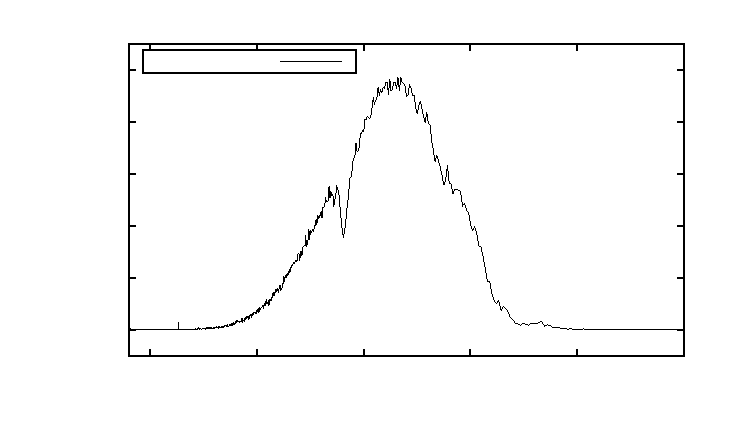
\includegraphics{halo-pbse-spec}}%
    \gplfronttext
  \end{picture}%
\endgroup

				\caption{}
				\label{fig:}
			\end{figure}
		
		% subsubsection gl_hlampenspektrum (end)
	
		\subsubsection{Absorbtionsspektren von Wasser und Benzol} % (fold)
		\label{ssub:absorbtionsspektren_von_wasser_und_benzol}

			\begin{figure}[htb]
				\centering
				% GNUPLOT: LaTeX picture with Postscript
\begingroup
  \makeatletter
  \providecommand\color[2][]{%
    \GenericError{(gnuplot) \space\space\space\@spaces}{%
      Package color not loaded in conjunction with
      terminal option `colourtext'%
    }{See the gnuplot documentation for explanation.%
    }{Either use 'blacktext' in gnuplot or load the package
      color.sty in LaTeX.}%
    \renewcommand\color[2][]{}%
  }%
  \providecommand\includegraphics[2][]{%
    \GenericError{(gnuplot) \space\space\space\@spaces}{%
      Package graphicx or graphics not loaded%
    }{See the gnuplot documentation for explanation.%
    }{The gnuplot epslatex terminal needs graphicx.sty or graphics.sty.}%
    \renewcommand\includegraphics[2][]{}%
  }%
  \providecommand\rotatebox[2]{#2}%
  \@ifundefined{ifGPcolor}{%
    \newif\ifGPcolor
    \GPcolorfalse
  }{}%
  \@ifundefined{ifGPblacktext}{%
    \newif\ifGPblacktext
    \GPblacktexttrue
  }{}%
  % define a \g@addto@macro without @ in the name:
  \let\gplgaddtomacro\g@addto@macro
  % define empty templates for all commands taking text:
  \gdef\gplbacktext{}%
  \gdef\gplfronttext{}%
  \makeatother
  \ifGPblacktext
    % no textcolor at all
    \def\colorrgb#1{}%
    \def\colorgray#1{}%
  \else
    % gray or color?
    \ifGPcolor
      \def\colorrgb#1{\color[rgb]{#1}}%
      \def\colorgray#1{\color[gray]{#1}}%
      \expandafter\def\csname LTw\endcsname{\color{white}}%
      \expandafter\def\csname LTb\endcsname{\color{black}}%
      \expandafter\def\csname LTa\endcsname{\color{black}}%
      \expandafter\def\csname LT0\endcsname{\color[rgb]{1,0,0}}%
      \expandafter\def\csname LT1\endcsname{\color[rgb]{0,1,0}}%
      \expandafter\def\csname LT2\endcsname{\color[rgb]{0,0,1}}%
      \expandafter\def\csname LT3\endcsname{\color[rgb]{1,0,1}}%
      \expandafter\def\csname LT4\endcsname{\color[rgb]{0,1,1}}%
      \expandafter\def\csname LT5\endcsname{\color[rgb]{1,1,0}}%
      \expandafter\def\csname LT6\endcsname{\color[rgb]{0,0,0}}%
      \expandafter\def\csname LT7\endcsname{\color[rgb]{1,0.3,0}}%
      \expandafter\def\csname LT8\endcsname{\color[rgb]{0.5,0.5,0.5}}%
    \else
      % gray
      \def\colorrgb#1{\color{black}}%
      \def\colorgray#1{\color[gray]{#1}}%
      \expandafter\def\csname LTw\endcsname{\color{white}}%
      \expandafter\def\csname LTb\endcsname{\color{black}}%
      \expandafter\def\csname LTa\endcsname{\color{black}}%
      \expandafter\def\csname LT0\endcsname{\color{black}}%
      \expandafter\def\csname LT1\endcsname{\color{black}}%
      \expandafter\def\csname LT2\endcsname{\color{black}}%
      \expandafter\def\csname LT3\endcsname{\color{black}}%
      \expandafter\def\csname LT4\endcsname{\color{black}}%
      \expandafter\def\csname LT5\endcsname{\color{black}}%
      \expandafter\def\csname LT6\endcsname{\color{black}}%
      \expandafter\def\csname LT7\endcsname{\color{black}}%
      \expandafter\def\csname LT8\endcsname{\color{black}}%
    \fi
  \fi
  \setlength{\unitlength}{0.0500bp}%
  \begin{picture}(6802.00,3968.00)%
    \gplgaddtomacro\gplbacktext{%
      \csname LTb\endcsname%
      \put(946,954){\makebox(0,0)[r]{\strut{} 0}}%
      \put(946,1454){\makebox(0,0)[r]{\strut{} 0.2}}%
      \put(946,1954){\makebox(0,0)[r]{\strut{} 0.4}}%
      \put(946,2453){\makebox(0,0)[r]{\strut{} 0.6}}%
      \put(946,2953){\makebox(0,0)[r]{\strut{} 0.8}}%
      \put(946,3453){\makebox(0,0)[r]{\strut{} 1}}%
      \put(1078,484){\makebox(0,0){\strut{} 400}}%
      \put(2047,484){\makebox(0,0){\strut{} 600}}%
      \put(3015,484){\makebox(0,0){\strut{} 800}}%
      \put(3984,484){\makebox(0,0){\strut{} 1000}}%
      \put(4952,484){\makebox(0,0){\strut{} 1200}}%
      \put(5921,484){\makebox(0,0){\strut{} 1400}}%
      \put(176,2203){\rotatebox{-270}{\makebox(0,0){\strut{}Intensität}}}%
      \put(3741,154){\makebox(0,0){\strut{}Wellenlänge $\lambda \ [\unit{nm}]$}}%
    }%
    \gplgaddtomacro\gplfronttext{%
      \csname LTb\endcsname%
      \put(2398,3530){\makebox(0,0)[r]{\strut{}Messwerte}}%
    }%
    \gplbacktext
    \put(0,0){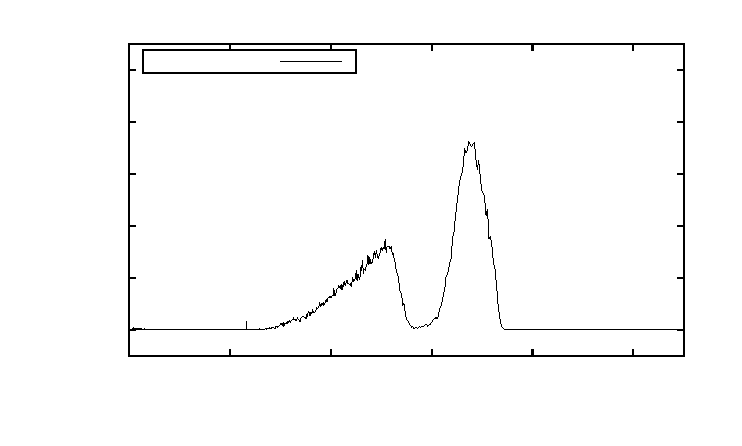
\includegraphics{halo-h20-spec}}%
    \gplfronttext
  \end{picture}%
\endgroup

				\caption{}
				\label{fig:}
			\end{figure}
		
			\begin{figure}[htb]
				\centering
				% GNUPLOT: LaTeX picture with Postscript
\begingroup
  \makeatletter
  \providecommand\color[2][]{%
    \GenericError{(gnuplot) \space\space\space\@spaces}{%
      Package color not loaded in conjunction with
      terminal option `colourtext'%
    }{See the gnuplot documentation for explanation.%
    }{Either use 'blacktext' in gnuplot or load the package
      color.sty in LaTeX.}%
    \renewcommand\color[2][]{}%
  }%
  \providecommand\includegraphics[2][]{%
    \GenericError{(gnuplot) \space\space\space\@spaces}{%
      Package graphicx or graphics not loaded%
    }{See the gnuplot documentation for explanation.%
    }{The gnuplot epslatex terminal needs graphicx.sty or graphics.sty.}%
    \renewcommand\includegraphics[2][]{}%
  }%
  \providecommand\rotatebox[2]{#2}%
  \@ifundefined{ifGPcolor}{%
    \newif\ifGPcolor
    \GPcolorfalse
  }{}%
  \@ifundefined{ifGPblacktext}{%
    \newif\ifGPblacktext
    \GPblacktexttrue
  }{}%
  % define a \g@addto@macro without @ in the name:
  \let\gplgaddtomacro\g@addto@macro
  % define empty templates for all commands taking text:
  \gdef\gplbacktext{}%
  \gdef\gplfronttext{}%
  \makeatother
  \ifGPblacktext
    % no textcolor at all
    \def\colorrgb#1{}%
    \def\colorgray#1{}%
  \else
    % gray or color?
    \ifGPcolor
      \def\colorrgb#1{\color[rgb]{#1}}%
      \def\colorgray#1{\color[gray]{#1}}%
      \expandafter\def\csname LTw\endcsname{\color{white}}%
      \expandafter\def\csname LTb\endcsname{\color{black}}%
      \expandafter\def\csname LTa\endcsname{\color{black}}%
      \expandafter\def\csname LT0\endcsname{\color[rgb]{1,0,0}}%
      \expandafter\def\csname LT1\endcsname{\color[rgb]{0,1,0}}%
      \expandafter\def\csname LT2\endcsname{\color[rgb]{0,0,1}}%
      \expandafter\def\csname LT3\endcsname{\color[rgb]{1,0,1}}%
      \expandafter\def\csname LT4\endcsname{\color[rgb]{0,1,1}}%
      \expandafter\def\csname LT5\endcsname{\color[rgb]{1,1,0}}%
      \expandafter\def\csname LT6\endcsname{\color[rgb]{0,0,0}}%
      \expandafter\def\csname LT7\endcsname{\color[rgb]{1,0.3,0}}%
      \expandafter\def\csname LT8\endcsname{\color[rgb]{0.5,0.5,0.5}}%
    \else
      % gray
      \def\colorrgb#1{\color{black}}%
      \def\colorgray#1{\color[gray]{#1}}%
      \expandafter\def\csname LTw\endcsname{\color{white}}%
      \expandafter\def\csname LTb\endcsname{\color{black}}%
      \expandafter\def\csname LTa\endcsname{\color{black}}%
      \expandafter\def\csname LT0\endcsname{\color{black}}%
      \expandafter\def\csname LT1\endcsname{\color{black}}%
      \expandafter\def\csname LT2\endcsname{\color{black}}%
      \expandafter\def\csname LT3\endcsname{\color{black}}%
      \expandafter\def\csname LT4\endcsname{\color{black}}%
      \expandafter\def\csname LT5\endcsname{\color{black}}%
      \expandafter\def\csname LT6\endcsname{\color{black}}%
      \expandafter\def\csname LT7\endcsname{\color{black}}%
      \expandafter\def\csname LT8\endcsname{\color{black}}%
    \fi
  \fi
  \setlength{\unitlength}{0.0500bp}%
  \begin{picture}(6802.00,3968.00)%
    \gplgaddtomacro\gplbacktext{%
      \csname LTb\endcsname%
      \put(946,954){\makebox(0,0)[r]{\strut{} 0}}%
      \put(946,1454){\makebox(0,0)[r]{\strut{} 0.2}}%
      \put(946,1954){\makebox(0,0)[r]{\strut{} 0.4}}%
      \put(946,2453){\makebox(0,0)[r]{\strut{} 0.6}}%
      \put(946,2953){\makebox(0,0)[r]{\strut{} 0.8}}%
      \put(946,3453){\makebox(0,0)[r]{\strut{} 1}}%
      \put(1283,484){\makebox(0,0){\strut{} 500}}%
      \put(2307,484){\makebox(0,0){\strut{} 1000}}%
      \put(3332,484){\makebox(0,0){\strut{} 1500}}%
      \put(4356,484){\makebox(0,0){\strut{} 2000}}%
      \put(5381,484){\makebox(0,0){\strut{} 2500}}%
      \put(6405,484){\makebox(0,0){\strut{} 3000}}%
      \put(176,2203){\rotatebox{-270}{\makebox(0,0){\strut{}Intensität}}}%
      \put(3741,154){\makebox(0,0){\strut{}Wellenlänge $\lambda \ [\unit{nm}]$}}%
    }%
    \gplgaddtomacro\gplfronttext{%
      \csname LTb\endcsname%
      \put(2398,3530){\makebox(0,0)[r]{\strut{}Messwerte}}%
    }%
    \gplbacktext
    \put(0,0){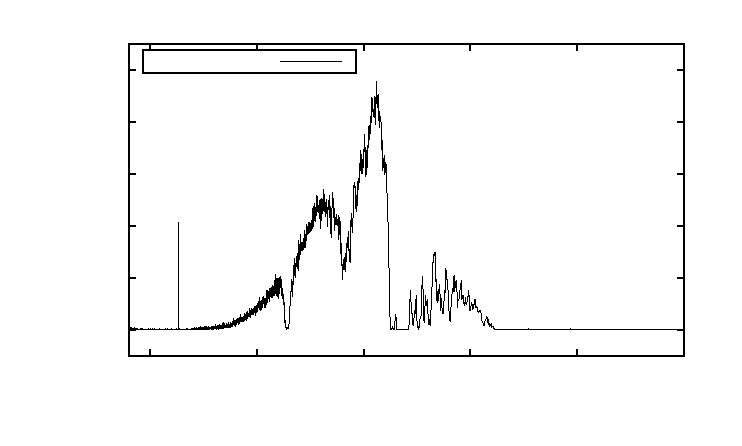
\includegraphics{halo-benz-spec}}%
    \gplfronttext
  \end{picture}%
\endgroup

				\caption{}
				\label{fig:}
			\end{figure}

		% subsubsection absorbtionsspektren_von_wasser_und_benzol (end)

	% subsection fourier_spektroskopie (end)

% section messwerte_und_auswertung (end)